%%
%% edengths.tex - LaTeX2e thesis driver
%%
%% Copyright (C) 1998 George Taylor
%% Copyright (C) 2010 Mathew Topper <damm_horse@yahoo.co.uk>
%%
%% This file is part of the University of Edinburgh, Department of
%% Engineering LaTeX2e thesis template.
%% 
%% The University of Edinburgh, Department of Engineering LaTeX2e thesis
%% template is free software: you can redistribute it and/or modify
%% it under the terms of the GNU General Public License as published by
%% the Free Software Foundation, either version 3 of the License, or
%% (at your option) any later version.
%% 
%% The University of Edinburgh, Department of Engineering LaTeX2e thesis
%% template is distributed in the hope that it will be useful,
%% but WITHOUT ANY WARRANTY; without even the implied warranty of
%% MERCHANTABILITY or FITNESS FOR A PARTICULAR PURPOSE.  See the
%% GNU General Public License for more details.
%% 
%% You should have received a copy of the GNU General Public License
%% along with the University of Edinburgh, Department of Engineering
%% LaTeX2e thesis template.  If not, see <http://www.gnu.org/licenses/>.
%%
%%
%%   ABOUT
%%
%% This is the driver file for a Latex2e template which corresponds to the
%% regulations regarding layout of a thesis submitted within the University
%% of Edinburgh school of Engineering. It is not `official', but conforms
%% as best as possible to the regulation as detailed at:
%%
%%   http://www.scieng.ed.ac.uk/Postgraduate/PhD/settingoutyourthesis.htm
%%
%% Please feel free to alter the template to your own liking, but note that
%% the template is made available under the GNU GPL and must be similarly
%% licenced should you wish to release your modified template.
%%
%%
%%   CREDITS
%%
%% This template is an amalgamtion of an existing Edinburgh University,
%% Electrical Engineering PhD Thesis class file (jthesis-v1.cls) authored by
%% George S Taylor which was released under the GNU GPL.
%% Code is included from the dmathesis class Written by M. Imran
%% for a thesis according to the university of Durham regulation, which was
%% released without copyright. It also contains ideas (possibly code) from the
%% Princeton thesis class file (PrincetonThesis.cls), authored by Mike Nolta.
%% Mathew Topper, Eoghan Maguire and Bill Edwards forsaw the need to maintain a
%% more recent latex implementation of the thesis regulations and thus, this
%% project was born. It is hoped that the template will be maintained by the
%% Edinburgh Engineering PhD community once released.
%%
%%
%%   RECORD OF REVISIONS
%%
%%     Date      Programmer        Description of change
%%     ====      ==========        =====================
%%   21/06/10    Mathew Topper     First Try.
%%
%%

%%%% LOAD DOCUMENT CLASS

\documentclass[crest,msfonts,fancychap,nopardent]{edengths}

%% Default report class options are:
%%
%% a4paper
%% openright - Start chapters on righthand side pages
%% titlepage - Title should be on it's own page

%% Standard available report class options are:
%%
%% 10pt
%% 11pt
%% 12pt
%% draft
%% final
%% fleqno
%% leqno
%% oneside
%% twoside

%% edengths class specific options:
%%
%% subsubnos - Enable numbering of subsubsections (note: these don't
%%             appear in the contents)
%% nosans    - Don't use the sans serif headers and captions
%% nopardent - Remove paragraph indent and add a line skip
%% msfonts   - Use MS fonts rather than latex default
%% fancychap - Use fancy chapter headings like jthesis
%% crest     - Use a crest on the front page
%% pdf       - Use pdflatex
%% labels    - Print labels in spine margin.

%% ADDITIONAL FORMATTING can be done in 'edengfmt.tex' where the page
%% dimensions, header/footers, table of contents and the names of 
%% the bibliography and list etc can be altered.
%% IN PARTICULAR THE LINE SPACING IS SET IN 'edengfmt.tex'

%% !!! NOTE: THE DEFAULT IS FOR LATEX NOT PDFLATEX !!!
%% !!!       USE 'pdf' OPTION FOR PDFLATEX         !!!

%%%% LOAD USER DEFINED PACKAGES.

%%
%% packages.tex - User defined packages for edengths.tex
%%
%% Copyright (C) 2010-2021 Mathew Topper <damm_horse@yahoo.co.uk>
%%
%%   ABOUT
%%
%% This file contains the user defined packages for a Latex2e template which
%% corresponds to the regulations regarding layout of a thesis submitted within
%% the University of Edinburgh.

%%%% PACKAGES AUTOMATTICALLY PROVIDED BY CLASS 
%%%%
%%%%  (No need to reload.  Options can be provided to these packages using the
%%%%   \PassOptionsToPackage command as per example at end.)

%% ifthen     -   Provides simple boolean commands

%% ifpdf      -   Detects whether pdflatex is being used.

%% graphicx   -   Allows inclusion of graphics in eps or jpg/pdf format

%% geometry   -   A more modern way of setting the page margins.
%%                'report' class options are passed automatically.

%% setspace   -   Define line spacing

%% appendix   -   Required for appendices

%% ae         -   Nicer pdf output using T1 fonts

%% fontenc    -   T1 encoding stops some errors for unknown fonts

%% titlesec   -   Custom chapter titles and page headers

%% caption    -   Custom formatting of captions

%% subcaption -   Use subfigures in captions and formatting of such.

%% tocloft    -   Allow modifications to the table of contents and lists

%% mathptmx   -   Option 'msfonts' to use these alternative font packages.
%% helvet         Note: you could add your own font packages in this file.

%% showlabels -   Print labels on the page if 'labels' option is given.

%% hyperef    -   Put clickable links into the document

%% hypcap     -   Links to figures show the figures rather than just the
%%                caption.

%% nomencl    -   Loaded with option 'nomencl' this provides a ``fly-by-wire''
%%                nomenclature indexing system. See chapter3.tex for an
%%                example.

%% xcolor     -   Loaded with option 'dvipsnames' with provides colors for pdf
%%                output. The options auto adjust for pdflatex and hyperref.
%%                See http://en.wikibooks.org/wiki/LaTeX/Colors for colours.

%%%%%%%%%%%%%%%%%%%%%%%%%%%%%%%%%%%%%%%%%%%%%%%%%%%%%%%%%%%%%%%%%%%%%%%%%%
%%%%%          Put ADDITIONAL packages you want to use here           %%%%
%%%%%%%%%%%%%%%%%%%%%%%%%%%%%%%%%%%%%%%%%%%%%%%%%%%%%%%%%%%%%%%%%%%%%%%%%%

%% Typset URLs properly. This package does automatic breaking of long URLs.
%% If you're using hyperref you dont need this but you might need the
%% 'breakurl' package depending on your compilation route.
%% Note: 'breakurl' must be the last package (which is normally 'hyperref').
\usepackage[hyphens]{url} 

%% AMS Math Packages
\usepackage{amsmath}
\usepackage{amssymb}
\usepackage{amsthm}

%% Fancy chemical symbols (Might require installation)
% \usepackage[version=3]{mhchem}

%% Better fractions ie 1/2 with diagonal slash
\usepackage{nicefrac}

%% Nicer tables
\usepackage{booktabs}

%% Citations
\usepackage[natbibapa]{apacite}

%% Proper hyphenation
\usepackage[british]{babel}

%% Rotating
\usepackage{pdflscape}

%% Paragraph control
\usepackage[defaultlines=4,all]{nowidow}


%%%%%%%%%%%%%%%%%%%%%%%%%%%%%%%%%%%%%%%%%%%%%%%%%%%%%%%%%%%%%%%%%%%%%%%%%%
%%%%%             Pass OPTIONS to packages you want here              %%%%
%%%%%%%%%%%%%%%%%%%%%%%%%%%%%%%%%%%%%%%%%%%%%%%%%%%%%%%%%%%%%%%%%%%%%%%%%%

%% Pass natbib the option 'numbers'
% \PassOptionsToPackage{numbers}{natbib}




%%%% LOAD USER DEFINED COMMANDS.

%%
%% defintns.tex - User defined commands for edengths.tex
%%
%% Copyright (C) 2010-2017 Mathew Topper <damm_horse@yahoo.co.uk>
%%
%%
%%   ABOUT
%%
%% This file contains the user defined commands for a Latex2e template which
%% corresponds to the regulations regarding layout of a thesis submitted within
%% the University of Edinburgh.

%%%%%%%%%%%%%%%%%%%%%%%%%%%%%%%%%%%%%%%%%%%%%%%%%%%%%%%%%%%%%%%%%%%%%%%%%%
%%%%%%%%%%             Define your commands here              %%%%%%%%%%%%
%%%%%%%%%%%%%%%%%%%%%%%%%%%%%%%%%%%%%%%%%%%%%%%%%%%%%%%%%%%%%%%%%%%%%%%%%%

%% New commands can be written using
%%    \newcommand{command}[inputs]{definition}.
%% In the definition the inputs are accessed with #1, #2, etc.
%%
%% If you want to override an existing command use \renewcommand instead
%% of \newcommand. \newcommand with give an error if command is already
%% defined.

%% If you are concerned that your command might override a default
%% you can use \providecommand which will ignore the new command if
%% a command of that name already exists.

%%%%% Some Example Maths Definitions (only use in maths mode)

\newcommand{\pdif}[2]{\frac{\partial #1}{\partial #2}}
%% ie \pdif{x}{t} would give partial x over t.

\newcommand{\dpdif}[2]{\dfrac{\partial #1}{\partial #2}}
%% inline partial derivative ie for $\dpdif{x}{t}$.
%% (\dfrac needs amsmath package)

\newcommand{\Ddif}[2]{\frac{D #1}{D #2}}
%% Material derivative

\newcommand{\spdif}[2]{\frac{\partial^{2} #1}{\partial #2^{2}}}
%% second partial derivative.

\newcommand{\altspdif}[3]{\frac{\partial^{2} #1}{\partial #2 \partial #3}} 
% mixed second partial i.e. \altspdif{x}{z}{t} = d2x / dzdt

\newcommand{\ndif}[2]{\frac{\mathrm{d} \, #1}{\mathrm{d} #2}}
%% ordinary differential.

\newcommand{\sndif}[2]{\frac{\mathrm{d} \,^{2} #1}{\mathrm{d} #2^{2}}}
%% ordinary second differential.


%%%% SET THE PATH FOR DIAGRAMS.

\graphicspath{{chapter1/}}%{/chapter3/}{chapter4/}
% {chapter_5/}{chapter_6/}{appendix/}}

%%%% PATH TO CREST

%% If you're not using the default crest files add the path here.
%% The default files are found in the 'front' directory.
%% Note: latex needs a eps file, while pdflatex needs pdf or jpg.
% \crestfile{/path/to/crest.pdps}

%%%% TITLE DETAILS

%% Author
\author{Robert Boberson}

%% Title
\title{Numerical Modelling of Flow
Past Submerged Bodies in the Presence of a Free Surface
With Some Other Crap}

%% Year of submission
\date{2010}

%%%% START DOCUMENT

\begin{document}

%%%% FRONT MATTER

%% The special formatting in the class requires the use of
%% a particular command to call the front matter (everything
%% before the table of contents). Just supply the path to the
%% file containing the front matter.

\makefrontmatter{front/frontmtr.tex}

%%%% TABLES AND LISTS

%% Table of contents
\tableofcontents

%% List of figure
\listoffigures

%% List of tables
\listoftables

%% List of figures and tables
% \listoffiguresandtables

%%%% START MAIN BODY TEXT

%% Call the edengths wrapper.
\startbody

\chapter{Introduction}

This is the beginning. I bet you wish that you had very started before long. I
shall now write two paragraphs. This is the second paragraph. In recent times
the way in which the human race uses and generates its energy has become of
extreme social, economical and environmental importance. Predictions of damaging
increases in mean global temperatures \citep[see][]{Solomon:2007:CUP} has
increased the need for carbon emitting energy technologies to be replaced by low
carbon alternatives. Additional long term economic factors are also playing
their part in shifting momentum to new technologies, in particular the concerns
about oil and natural gas supplies. Demand for oil and gas is expected to
outstrip supply within the current century, leading to inflated prices and
energy security issues. Unfortunately, although the resource and environmental
issues are occurring simultaneously, they are not necessarily mutually
supportive. For instance, once the price for oil has reached a certain value it
can be economically synthesised from coal, providing no environmental benefits.
In fact, if the market were left to choose a method for replacing dwindling oil
resource then this is one of the most likely substitutes; even in light of
population growth, coal reserves are estimated to last for hundreds of years
\citep[see][]{Jaccard:2005:CUP} and thus the cost is low.

With markets failing to deliver the necessary changes, it has become the
responsibility of governments to intervene under the premise that the predicted
environment and economical consequences of inaction will outweigh the costs
incurred by immediate action. This is a tough political task as, particularly in
the UK, energy markets have followed a trend of liberalised trading which makes
strategic decision making extremely challenging. Private investment is unlikely
to match policy, unless the policy is seen to be long term and economically
advantageous; a virtual impossibility when scientific and economic opinions of
the market requirements are so uncertain. In addition, the likelihood of direct
governmental intervention in the form of capital investment is now looking more
unlikely, due to the recent financial crisis. Capital spending is set to fall
significantly in order to reduce deficits endured to rescue the banking sector.

Despite the potential funding problems, the United Kingdom (UK) Government's
Climate Change Act 2008 \citep*[see][2008]{CCA:2008:Defra} introduced for the
first time legally binding targets for greenhouse gas emissions from within the
UK. The targets set an 80\% reduction of greenhouses gases by 2050 and a 26\%
reduction of carbon-dioxide $\text{CO}_{2}$ emissions by 2020 with respect to
1990 levels. This is set in the context of Britain's pre-existing target to
reduce emissions by 12\% as a ratified signatory of the Kyoto Protocol
and a European Union proposal to cut EU wide greenhouse gas emissions by 20\% by
2020 each with respect to 1990 levels. Electricity generation in the United
Kingdom accounts for 37\% of all emissions and as part of the
government's greenhouse gas reduction strategy it will seek to reduce this to
zero by 2030 \citep[see][2008]{CCC:2008}. Given the enormity of this task it is
foreseen that a varied mix of low/zero carbon electricity generating
technologies will be required.
\begin{quote}
 ``It is a well known fact that the use of a high-order panel method is more
accurate than the
low-order panel method or the discrete vortex method in computing the velocity
field as the
appearance of instabilities in the vortex sheet due to the spurious numerical
effects introduced by
a too-crude representation.''
\end{quote}
As such, a melting pot of renewable and sustainable energy technologies have
begun to compete to become part of a `post-carbon' energy mix. Some of these
technologies are well established, such a nuclear, biomass and wind, others less
so, such as solar photovoltaic and marine energy. In addition, carbon emitting
technologies such as coal remain an attractive option for governments and
investors alike, as carbon capture and storage technology promises to store away
the greenhouse gases emitted in combustion. However, carbon capture and storage
is still an unproven technology and thus, the future costs of this and many
other of the new energy technologies are hard to predict and are, at present,
highly contestable; ultimately, over the long term, energy cost is the most
likely deciding factor as to which technologies will feature most. Hence, each
industry is working hard to reduce costs via research and innovation.

%\chapter{Another Chapter}

\section{The first section}

Note that all section and chapter titles should use lower case except
for the first character of the first word. Here is a reference to a
paper~\cite{apaper}. Figure~\ref{fig:picture} is a weird picture.

\begin{figure}[h]
  \centering
  %% Because graphicspath was set in edengths.tex you only need to
  %% supply the file name here, i.e. examplepicture (doesn't need the
  %% extension) and not the full path. Just remember to add the path
  %% to \graphicspath{{thispath/}{thatpath/}}
  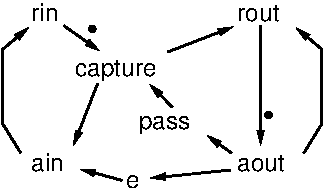
\includegraphics[width=2in]{examplepicture}
  \caption[Long caption and \textit{some italics} to see what happens]%
  {This is an example of pdf with a very long caption and \textit{some italics} to see what happens and it should see what happens over two lines.}
\label{fig:picture}
\end{figure}

\subsection{A subsection}

Lorem ipsum dolor sit amet, consectetur adipiscing elit. Maecenas nec orci lacus, ac sollicitudin tortor. Maecenas rutrum vestibulum rhoncus. Vestibulum non ligula nibh. Cum sociis natoque penatibus et magnis dis parturient montes, nascetur ridiculus mus. Phasellus egestas sodales lacus, ac scelerisque nulla venenatis sed. Ut elementum turpis ac lacus consectetur consequat. Sed at est eros. Praesent erat velit, dictum id adipiscing eu, ultrices vel nisi. Nullam at nisl ut est posuere commodo tincidunt eget nisl. Integer id erat non metus adipiscing dignissim quis sed enim. Curabitur viverra lobortis eleifend. Proin vestibulum nunc eu augue dapibus quis porttitor ipsum rhoncus. Duis tortor tellus, suscipit sit amet ornare id, lacinia sed lacus. Ut in molestie ligula. Praesent euismod lectus vitae arcu malesuada tempus. Aliquam pharetra tincidunt augue in eleifend. Curabitur porttitor vulputate quam, ut fringilla mauris porta eu. Curabitur sodales, felis non vestibulum feugiat, urna diam bibendum purus, ac scelerisque massa eros sit amet ipsum. In elementum laoreet aliquam.

\subsubsection{A subsubsection}

Aliquam eget sapien tellus, sed rutrum leo. Vestibulum et quam sit amet dolor gravida sagittis. Aenean dapibus urna a nibh sollicitudin pharetra. Sed nisi augue, vehicula sed tristique facilisis, lacinia ut augue. Nam quis tempor mi. Vestibulum lorem leo, aliquet at sollicitudin vitae, fringilla id odio. Aenean a orci odio. Mauris tincidunt eros ac libero suscipit molestie. Donec feugiat turpis a urna suscipit in pellentesque magna pretium. Vivamus eget nunc vitae nunc ultricies tincidunt. Duis dictum eros et lorem auctor id ullamcorper diam commodo. Pellentesque quis dolor nec urna vestibulum pellentesque. Donec luctus mi ut nisi hendrerit pulvinar. Donec fringilla, lectus vitae accumsan sollicitudin, sem metus mollis risus, nec laoreet ante arcu ut augue.

\subsection{Another subsection}

Table~\ref{tab:atable} is an example of a~\footnote{this is a
footnote} simple table.

\begin{table}[htb]
\begin{center}
\begin{tabular}{|c|c|c|}
\hline
1.0 & 2.0 & 3.0 \\
\hline
4.0 & 5.0 & 6.0 \\
\hline
\end{tabular}
\caption{A table}
\label{tab:atable}
\end{center}
\end{table}


\section{Another section}

This is a long and boring paragraph for the purpose of testing the
spacing between paragraphs and the use or otherwise of indentation. I
think a space between paragraphs and without the first line indented
is somewhat easier to read than no space between paragraphs and with
the first line indented.

Another equally exciting paragraph, one two three four five six seven
eight nine ten eleven twelve thirteen fourteen fifteen sixteen
seventeen eighteen nineteen twenty and so on.

\begin{equation} \label{eqn:dct}
z(k,l) = \frac{2}{N} \alpha(k) \alpha(l) \sum_{m=0}^{N-1} \sum_{n=0}^{N-1}
         x(m,n) \cos \frac{ (2m+1) \pi k}{2N} \cos \frac{ (2n+1) \pi l}{2N}
\end{equation}

\begin{equation} \label{eqn:idct}
x(m,n) = \frac{2}{N} \sum_{k=0}^{N-1} \sum_{l=0}^{N-1}
         \alpha(k) \alpha(l) z(k,l)
\end{equation}

\begin{quotation}
This is a quotation, another equally exciting paragraph, one two three
four five six seven eight nine ten eleven twelve thirteen fourteen
fifteen sixteen seventeen eighteen nineteen twenty and so on. Just
checking it is single spaced.
\end{quotation}

%\frontchapter{Nomenclature}

\section*{Main equations}
\begin{equation}
  a=\frac{N}{A}
\end{equation}%
\nomenclature{$a$}{The number of angels per unit area}%
\nomenclature{$N$}{The number of angels per needle point}%
\nomenclature{$A$}{The area of the needle point}%
The equation $\sigma = m a$%
\nomenclature{$\sigma$}{The total mass of angels per unit area}%
\nomenclature{$m$}{The mass of one angel}
follows easily.

%\include{chapter4/chapter4}
%\include{chapter5/chapter5}
%\include{chapter6/chapter6}

%%%% START APPENDICIES

%% Call the edengths wrapper.
\startappendix

\chapter{Collocation Method at the Wake Edges}
\label{append:collocation}

\setcounter{equation}{0}

A collocation based gradient method is formulated in \citet[sec. 5]{Gray:2004:SJoSC}. In that
paper it is proved that the method, although applicable to a general Laplace problem, is not
applicable to the crack problem. The difficulty arises from an additional constant in the shape
functions for the most singular point. However, the zero value of 

% To finalise the applicability of this method, prior to its derivation, and in respect to the
% necessity of an internal and external domain, it is proposed that the method does not suffer the
% same difficulties at an edge as the Galerkin method.
% 
% To prove this consider a general point of interest lying on either the top and bottom
% surfaces of the wake, $S^{+}$ and $S^{-}$. Once more, the average of the velocities of the top and
% bottom are saught. This is written as
% \begin{multline}
% \frac{1}{2} \left( \pdif{\phi^{+}}{E_{k}} + \pdif{\phi^{-}}{E_{k}} \right) = \left\{ \lim_{\pint
% \rightarrow P} - \lim_{\pext \rightarrow P}
% \right\} \int_{S} \phi \frac{\partial^{2}G}{\partial\E_{k}\partial\n} \: dS \\
% = \left\{ \lim_{\pint \rightarrow P} - \lim_{\pext \rightarrow P}
% \right\} \int_{S^{+}} \phi^{+} \frac{\partial^{2}G}{\partial\E_{k}\partial\n^{+}}
% \: dS + \int_{S^{-}} \phi^{-} \frac{\partial^{2}G}{\partial\E_{k}\partial\n^{-}}
% \: dS
% \end{multline}
% Moving on to considering a point lying on the division between $S^{+}$ and $S^{-}$, the above
% becomes
% \begin{equation}\label{eq:edge_collocation}
% \pdif{\phi}{E_{k}} = \left\{ \lim_{\pint \rightarrow P} - \lim_{\pext \rightarrow P}
% \right\}
% \int_{S^{+}} \phi^{+} \frac{\partial^{2}G}{\partial\E_{k}\partial\n^{+}} \: dS +
% \int_{S^{-}} \phi^{-} \frac{\partial^{2}G}{\partial\E_{k}\partial\n^{-}} \: dS
% \end{equation}
% given that $\phi^{+} + \phi^{-} = \phi$. The difference between the internal and external limits
% will cancel all of the non-singular integrals, hence the remaining integrals are just the singular
% ones in $S^{+}$ and $S^{-}$. The right hand side of equation~\eqref{eq:edge_collocation} can
% easily be combined into a single surface by

The development of the collocation method is very similar to that of the edge adjacent integral,
expect that only one polar transformation is available. To begid
effect of
differ


% END OF CHAPTER

%%%% WRITE OUT BIBLIOGRAPHY

%% Path to bib file.
\bibliography{bib/edengref}{}

%% Path to style file. It's recommand you use the provided style file
%% (a variation on plainnat) as it does italic et als and reduces
%% all first names to initials.
\bibliographystyle{bib/edengnat}

\end{document}
